%
\newglossaryentry{X}
{
  type=genericmath,
  name={$\ensuremath{X} $},
  description={Set of locations for a user. ($R^2$)},
}
\newglossaryentry{Z}
{
  type=genericmath,
  name={$\ensuremath{Z} $},
  description={For every $x \in X$ a perturbed location $z \in Z$ is reported.},
}
\newglossaryentry{privacy level}
{
  type=genericmath,
  name={$\ensuremath{l} $},
  description={Privacy level},
}
\newglossaryentry{radius}
{
  type=genericmath,
  name={$\ensuremath{r} $},
  description={Radius},
}
\newglossaryentry{Epsilon}
{
  type=genericmath,
  name={$\ensuremath{\epsilon} $},
  description={Defined as $\epsilon = l/r$},
}
\newglossaryentry{theta}
{
  type=genericmath,
  name={$\ensuremath{\theta} $},
  description={Angle},
}
\section{2D-Laplace}
The idea of \gls{gi} was introduced to address the issue of privacy and location data \citep{DBLP:journals/corr/abs-1212-1984} (See Equation \ref{algo:2d-geo-indistinguishability}).
It offers an alternative approach for achieving (local) differential privacy for geographical data (latitude/longitude).
The mechanism achieves this by locally adding noise to the location before sending it to a location-based system (LBS).
This section starts with an introduction to mathematics, and for each of the different subsections, we visualize and explain open challenges and theoretic for applying them for clustering.
%\glsaddall
%\leading{10pt}
%\printglossary[type=genericmath, nonumberlist]
%The other symbols can be found in section \ref{section:dp}.
\subsection{Planar and polar Laplace}
In section \ref{theory:geo-indistinguishability}, an explanation of the concept of \gls{gi} has been given.
As indicated, the method works on 2-dimensional data, and when visualized, this can be done with a so-called plane \citep{DBLP:journals/corr/abs-1212-1984}.
From there, the term "Planar" Laplace (2D-Laplace) originated and was used thoughtfully by Andres et al.

The idea of 2D-Laplace is to generate an area around $x0 \in X$ according to the multivariate Laplace distribution.
The mechanism of 2D-Laplace is a modification of the Laplace algorithm to support distance \citep{DBLP:journals/corr/abs-1212-1984}.
This distance method $dist(x, x')$ is a method to calculate the Euclidean distance between two points $x$ and $x'$.
Recalling the definition of Laplace, this method $|x-x'|$ is replaced by the distance metric.
Hence, the definition of the \gls{pdf}) by Andrés et al. is:
\begin{equation}
  \frac{\epsilon^2}{2*\pi}e(-\epsilon d(x_0, x))
  \label{eq:polar-laplace-pdf}
\end{equation}
Which is the likelihood a generated point $z \in Z$ is close to $x0$.
The method works for Cartesian coordinates but was modified to support polar coordinates by including $\theta$.
So each point is reflected as $(r, \theta)$.
A point $z \in Z$ where $z = (r, \theta)$ is randomly generated using two separate methods for calculating $r$ and $\theta$.
This idea is visualized in the following figure:
\begin{figure}[H]
  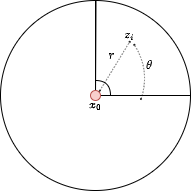
\includegraphics[scale=0.6]{TheorethicalFramework/ND-Laplace/Images/polar-laplace.png}
  \centering
  \caption{Representation of the generated $z = {r \theta}$ and original point $x0$.}
  \label{figure:parea}
\end{figure}

\textbf{Calculating $r$:}
This variable is defined as $dist(x_0, z)$ and can be randomly drawn by inverting the \gls{cdf} for the Laplace distribution:
\begin{equation}
  C{_\epsilon}{^{-1}}(p) = - \frac{1}{\epsilon}(W_-1 (\frac{p - 1}{e}) + 1)
\end{equation}
For this equation, $W_{-1}$ is a Lambert W function with a -1 branch.
\todo[inline]{Explain -1 branch?}
The Lambert w function (also called the product logarithm) is defined as $W(x)e^{W(x)} = x$ \citep{lehtonen_lambert_2016}.
The purpose of the Lambert w function is to invert the \gls{cdf} of the Laplace distribution to generate random noise for one of the coordinates ($r$) using the random value of $p$.

\textbf{Calculating $\theta$:}
The other variable ($\theta$) is defined as a random number $[0, 2\pi]$. \newline
To visualize the data, it is necessary to convert the polar coordinates for $z = (r, \theta)$ back to planar coordinates $z = (x, y)$.
This conversion is described as step 4 of the planar Laplace algorithm \citep{DBLP:journals/corr/abs-1212-1984} and visualized using figure \ref{figure:geo}.
\begin{figure}[h]
  \includesvg[width=0.8\textwidth]{TheorethicalFramework/ND-Laplace/Images/polar-laplace-to-planar.svg}
  \centering
  \caption{Representation of converting the perturbed point $z = (r, \theta)$ to a point ${z_x, z_y}$}
  \label{figure:geo}
\end{figure}

\newpage
\subsection{Truncation} \label{theory:truncation}
After adding the noise to the data, it cannot be ensured the data is within the original domain (figure \ref{figure:truncation-2d}).
If this is not the case, the data is easily distinguished by an unwanted adversary \citep{DBLP:journals/corr/abs-1212-1984,9646489}.
The truncation is an essential part of the mechanism to ensure the data is contained within the domain of the original data $X$.
%We assume a user has a set of data points with a range of [-1, 1].
\begin{figure}[H]
  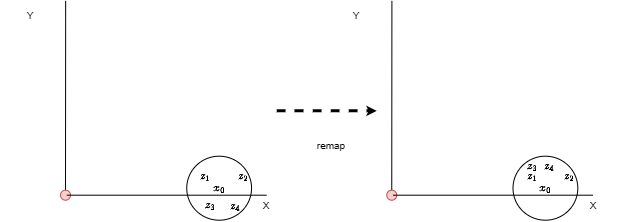
\includegraphics[width=0.7\textwidth]{TheorethicalFramework/ND-Laplace/Images/remapping.png}
  \caption{Representation of truncation of data points for 2-dimensional Laplace mechanism.}
  \label{figure:truncation-2d}
\end{figure}
%A solution was described by Andres et al. in step 5 of the Laplacian mechanism for 2D space \citep{DBLP:journals/corr/abs-1212-1984}.
%A viable solution is to create a grid around the diameter of the set of points $X = R^2$ that belong to the user \citep{DBLP:journals/corr/abs-1212-1984}.
The approach Andres et al. introduces is to remap a perturbed point $z$ to the closest point $x'$ in $G$ \citep{DBLP:journals/corr/abs-1212-1984}.
Here, $G$ is a grid generated using constant cell width.
%Although this approach remaps data within the original domain of $X$, it is not guaranteed it preserves \gls{gi} anymore.
Let the below equation be the collection of probabilities for a point being remapped to a grid cell $x'$ \citep{DBLP:journals/corr/abs-1212-1984}:
\begin{equation}
  R(x) = { y \in R^2 | \forall x' \in G \cdot d(y, x') \leq d(y, x')}
  \label{eq:grid-probability}
\end{equation}
The original \gls{gi} definition contains $K$, which is the probability of $z$ being reported as $x$ (See Equation: \ref{theory:geo-indistinguishability}).
However, this probability is no longer guaranteed because $z$ can also be part of $G$ \citep{DBLP:journals/corr/abs-1212-1984}.
Hence the probability is now $R_X(x) = R(x) \cup X$. \newline
So, the $R_X(x)$ has a different shape depending on the distance $x_0$ and $x'$ (ergo, it depends on the grid cell width). This is due the step units of $G$ stay the same, while the distance $r$ grows \citep{DBLP:journals/corr/abs-1212-1984}.
\newpage
To overcome this issue, Andres et al. propose a way of calculating $\epsilon'$, depending on the step-unit $u$. \citep{DBLP:journals/corr/abs-1212-1984}.
They proved this in theorem 4.1 \citep{DBLP:journals/corr/abs-1212-1984}:
\begin{theorem}[Discretization 2D-Laplace]
  Assume $r_{max} < \frac{u}{\delta_{\theta}}$, and let $q = \frac{u}{r_{max}}\delta_{\theta}$. Let $\epsilon$, $\epsilon' \in R^+$ such that \\
  $\epsilon' + \frac{1}{u}ln \frac{q + 2 e^{\epsilon'u}}{q - 2 e^{\epsilon'u}} \leq \epsilon$ \\
  Then $K_{\epsilon'}$ provides $\epsilon$-geo-indistinguishability within the range of $r_{max}$. Namely, if ${d(x_0, x), d(x'_0, x) \leq r_{max}}$ then: \\
  $K_{\epsilon'}(x_0)(x) \leq e^{\epsilon d(x_0, x'_{0})} K_{\epsilon'}(x'_{0})(x)$.
  \label{theorem:discretization}
\end{theorem}
Here, $\delta_{\theta}$ is the machine's precision, which is the hardware precision of the GPS-location in the context of geographical data. We will omit this in our research, but still provide the full theorem nonetheless. 
The theorem states that $\epsilon'$ is the additional noise needed to satisfy \gls{gi} with the introduction of discretization.
%Then, the final step is truncation based, which is based on the discretization \citep{DBLP:journals/corr/abs-1212-1984}.
It is sufficient to take $r_{max}$ as $diam(X)$, which is the diameter of the set of points $X$ if it satisfies theorem \ref{theorem:discretization} \citep{DBLP:journals/corr/abs-1212-1984}:
So, $r_{max}$ is the maximum distance between points in $X$, which is the area where geo-indistinguishability can be guaranteed \citep{9646489}.

\mycomment{In the context of our research, it is more convenient to find the $u$ based on a given $\epsilon$.
So the challenge is to find the $u$ that satisfies \gls{gi}.
This can be solved by finding the root of the function:
\begin{equation}
  \epsilon' + \frac{1}{u}ln (\frac{\frac{u}{r_{max}} + 2 e^{\epsilon'u}}{\frac{u}{r_{max}} - 2 e^{\epsilon'u}}) - \epsilon = 0
  \label{eq:find-u-with-epsilon}
\end{equation}
The idea of finding the root of a function is to try different values of $u$ until $f(u) = 0$. \todo{Have some proof}
\todo[inline]{Maybe extend this with some more explanation?}}
%This idea was later improved by Chatzikokolakis et al., introducing an optimized way of remapping \citep{chatzikokolakis_efficient_2017}.
%The algorithm uses the Bayesian rule to minimize the loss of utility while remapping the data.
%Instead of remapping to the closest point, it remaps to a location where the loss is minimal.
%To decrease the performance impact of this algorithm, it is possible only to consider a specific region around the perturbed point $z$.
%The disadvantage of this method is the need for a prior set of data points to calculate the optimal remapping.
%It does not work for new users and extends the training period.

\mycomment{\subsection{Optimizing for clustering} \label{2d:optimizing}
The decision of the parameters for the algorithm is straightforward as it depends on the $\epsilon$. \label{paragraph:choosing-r}
This constant is calculated by defining the radius $r$, and the desired level of privacy $l$ and $\epsilon$ is calculated using $l/r$.
The $l$ is a predefined constant $l \in R^+$ but usually will be below 10.
For geographical data, the $r$ can be configured using meters as a unit of measure.
So, for example, $r = 200$ corresponds to a radius of 200m around point $x_0$.
Without a unit, it is a challenge to define a reasonable radius.
%The $\epsilon$ can be considered the inverse unit of $r$ \citep{DBLP:journals/corr/abs-1212-1984}.
In that regard, the radius can also be a flexible value defined based on the crowdedness of a region \citep{chatzikokolakis_constructing_2015}.
Suppose a user's location is within a crowded area.
In that case, the radius can be smaller than if the user is located in a rural area (because the user's location is indistinguishable due to the overlap of other users' locations).
Instead of providing \gls{gi}, the authors introduce a more flexible privacy definition $d_x$-privacy.
The $r$ is calculated based on the mass of other regional locations $r$, which they call \emph{privacy mass}.
So, the total mass of a set A is defined as $M(A) = \sum_{x \in A} m(x) = a + q(x)b$.
Where $m(x)$ is the mass of a location $x$ and $x$ is in value [0, 1].
For this formula, $a$ is the number of points assigned to each location.
The authors define $q(x)$ as the "quality" of a point, which is essentially the number of other users that are also interested in the same point (e.g. a mall).

The $a$ is defined as a Euclidean ball $B_r = {x' | d_{euc}(x, x') \leq r}$, which returns all locations within the radius $r$.
\todo[inline]{Explain this formula better, and create it as a separate equation}
To retrieve a value within [0, 1], the authors use the following formula:
\begin{equation}
  a = \frac{1}{|B_r|}
  \label{equation:privacy-mass-a}
\end{equation}
If the locations are only considered for space and not quality, $q(x)$ is defined as 0 \citep{chatzikokolakis_constructing_2015}.

Although the method is an interesting approach to increasing utility while not reducing privacy, it is hard to adopt for clustering.
For applying it for \gls{ldp}, it is required to supply each user with prior knowledge of the dataset.
This approach would require interaction between data points, hence an interactive setup of the mechanism instead of a non-interactive one. \newline
Nonetheless, the idea of using crowded locations is an exciting approach that is researched further in section \ref{theory:privacy-utility-nd}
}


\newpage
\subsection{Final mechanism}
Finally, we provide as means of a summary the final algorithm for the Laplace mechanism for 2D space
\begin{algorithm}[H]
  \caption{Full mechanism for perturbing training data for 2D-clustering using planar/2D-Laplace \citep{DBLP:journals/corr/abs-1212-1984}}\label{alg:rq1}
  \begin{algorithmic}
    \Require $x \in X$  \Comment 2D array of points \\
    $\epsilon$ \Comment should satisfy Theorem \ref{theorem:discretization}
    \Ensure $z \in Z$ \Comment 2D array of perturbed points
    %\State $r = \frac{\sigma}{2}$ \Comment formula 4.1
    %\State $\epsilon = \frac{l}{r}$ \Comment Calculating privacy budget \citep{DBLP:journals/corr/abs-1212-1984}
    \State $x_{min} \gets min(X)$
    \State $x_{max} \gets max(X)$
    \State $Z \gets []$
    \For{$point_i \in X$}
    \State $\theta \gets [0, \pi2]$       \Comment Random noise for $\theta$
    \State $p \gets [0, 1]$
    \State $z_i \gets C{_\epsilon}{^{-1}}(p)$       \Comment formula 3.2
    %\State $z_i \gets T(x_{min}, x_{max}, point_i, z_i)$ \Comment algorithm 1.
    \State $x_{perturbed} \gets point_{i_x} + (z_{i_x} * \cos(\theta)) $ \Comment add noise to x-coordinate
    \State $y_{perturbed} \gets point_{i_y} + (z_{i_y} * \sin(\theta)) $ \Comment add noise to y-coordinate
    \State append $x_{perturbed}, y_{perturbed}$ to Z
    \EndFor
    \State \Return Z
  \end{algorithmic}
  \label{alg:2d-laplace}
\end{algorithm}
\newpage